\chapter{Package improvements implementation}
\label{ch:implementation}

\section{Administration requirements}
One of the administrator's main tasks while managing networks is, if required, to facilitate the coexistence of different Routing protocols in the same network section. Hence the requirement of rich routing tools as Quagga or Bird to act as facilitators of this route \textit{crossed-announcement} -and even attributes translation- between protocols.

Administrators require:
\begin{itemize}
    \item A full-featured tool with an easy and intuitive UI to manage and monitor protocol health and data efficiently and avoiding any handmade/custom edit, reducing configuration's complexity.
    \item Use of LEDE/OpenWRT-based firmwares widely used in the target network.
    \item A Routing protocols management tool that, at least, supports BGP Static Routing Protocol and it is able to share routes with BMX6 Dynamic Routing Protocol in a manageable way.
    \item Use Bird Daemon instead of Quagga to make us of its proven efficiency, low resource consumption and powerful filter capabilities, which is critical to some of the widely used commodity hardware in Guifi.net.
    \item Use and improve Bird Daemon's configuration integration package (bird-uci and luci-app-bird) available in the official Routing Repository of LEDE/OpenWRT.
    \item Avoid project-specific customisations in the integration package that would not benefit all the community. If required, add those custom enhancements in a development branch.
    \item Update Package's documentation and create new topics to cover Web UI interface and any manual process not covered by package's improvements.
    \item Update Bird integration package in order to be compliant to the latest API (v1.6.3 when this document was written).
    \item Enhance Web UI to support user-friendly configuration and visualisation of the following:
    \begin{itemize}
        \item Bird Daemon service status
        \item Bird Daemon events information (Logs)
        \item Filters and Functions editing using an embedded HTML text editor.
        \item Update old configuration Web pages, fix some outdated options and re-sort them to a more logically order.
    \end{itemize}
    \item Do theoretical viability investigation to use uBus Daemon as a mechanism to communicate with Bird Daemon and get health information and current-status information for handled protocol using JSON messages.
\end{itemize}

\section{Changes and improvements implemented}
The following sections summarises what has been changed as part of this project's development, which changes have been successful, challenges found and lessons learnt that will help towards future versions of the Package.

\subsection{Build and deployment process documentation update}
One of the first challenges I found during the initial investigation was that the documented process for building the package was wrong. This misalignment led into few days testing the build process using the latest version of the development environment in order to tune it (the original building process was documented in 2014).

\begin{itemize}
    \item Generalise Makefiles (bird4/bird6) and post installation scripts.
    \item Add detailed steps to get Package's source, add bird required packages into the Image Build settings, compile it (\texttt{make}) and deploy it in the target router.
    \item Add alternative mechanisms, Package information and (after finishing changes in the Package), Package known issues.
\end{itemize}

\subsection{Apply code standards}
As a daily Bash user, one of the main concerns that I had once I did retake the project was the state of the code because I did stop giving support to the Package on 2014 and I have improved drastically my consciousness towards clean, standard and following-best-practises code. Therefore, the top priority task I got was to normalise the code, apply best practises and, where possible, refactor it to follow a \textit{library}-pattern to be able to formalise an API and, in future releases, even to create unitary tests that would automate Package's tests.

The first challenge I found was that LEDE/OpenWRT firmwares use the light compound of Linux tools BusyBox\footnote{\href{https://busybox.net/downloads/BusyBox.html}{BusyBox}: light and optimised UNIX tools including most of the widely used terminal commands (i.e. \texttt{ash}, \texttt{cat} or \texttt{rm}).}. This all-in-one tool comes really handy in embedded environments where performance and storage are critical but some of its tools are limited versions of the original ones.

Particularly, the tool that has been more challenging is \textit{ash}, which is the built-in Shell Command Line included instead of \textit{Bash} and, although it includes most of its features, there are few others like Arrays that are not available and requires the developer to re-think the solution (Ash readme page suggest the use of \texttt{set} command).

Some examples of the improvements applied are:
\begin{itemize}
    \item Encapsulate variables with curly brackets to avoid wrong substitutions or other common issues where mixing variable names and other strings:
    \begin{lstlisting}[language=bash,caption={Variable encapsulation}]
root@LEDE:~# path="/etc/"
root@LEDE:~# ls $pathconfig/bird4
ls: /bird4: No such file or directory
root@LEDE:~# ls ${path}config/bird4
/etc/config/bird4
\end{lstlisting} 
    This is a forced example but there are some instances where, in really complex scripts, unexpected substitutions could happen.
    \item Encapsulate Strings appropriately to avoid unexpected substitutions or code execution (i.e. script injection): this is an uncommon situation that could happen with commands like \texttt{sed}, where quotes and other special symbols are crucial to get the expected output.
    \item Use of 4 spaces instead of tabs for code readability.
    \item Use of simplified \texttt{if} statements \textbf{only} with clear and single-line occasions. Avoid using simplifications on instances where more than one line is required or the command is too large and would be more reasonable to split it using backslash (\texttt{\textbackslash}).
    
Acceptable:
\begin{lstlisting}[language=bash,caption={If statement simplification (I)}]
root@LEDE:# var="true"
root@LEDE:# [ "$var" = "true" ] && install_package="y" || install_package="n"
var is true
\end{lstlisting}
Unacceptable:
\begin{lstlisting}[language=bash,caption={If statement simplification (II)}]
root@LEDE:# [ "$(uname)" = "Linux" ] && { . /etc/os-release;
 echo -e "\n $LEDE_RELEASE \n"; } || echo "Not Available"

LEDE Reboot SNAPSHOT r3969-8322dba

root@LEDE:#
\end{lstlisting}
\end{itemize}

\subsection{init.d script and service management}
\label{sec:initd}
Bird's init.d script (\texttt{/etc/init.d/bird4}) manages the service on boot or on demand. Bird Daemon's init.d file is substituted on installation time by \texttt{/etc/bird\{4|6\}/init.d/bird\{4|6\}} script, and the original one backed up as \texttt{/etc/bird\{4|6\}/init.d/bird\{4|6\}.orig} to be restorable in the event of uninstalling the Package.

Improvements introduced are:
\begin{itemize}
    \item Refactor init.d script and split it in two files. \texttt{bird\{4|6\}} for service management and \texttt{bird\{4|6\}-lib.sh} as an \textit{API/function} holder for UCI-bird configuration translation.
    \item Store a backup of the current configuration each time the service is started. However, this backup is overwritten each time and it is administrator decision to take a copy of this file before reloading the service.
    \item Add \textit{smart} service management to avoid multiple start/stop/restart calls to the service, causing service disruptions if not required (i.e. multiple start calls should be ignored). See figure \ref{fig:initdt}.
    \item Add extra management functions for LUCI Web management. These new functions call the original ones but forcing plain text outputs. See figure \ref{fig:initdui}.
    \item Re-sort UCI translation script's in order to fix an issue with Functions and Filters.
    \item Enhance service handling and error information logging, previously dismissed.
\end{itemize}

\begin{figure}[ht!]
    \centering
    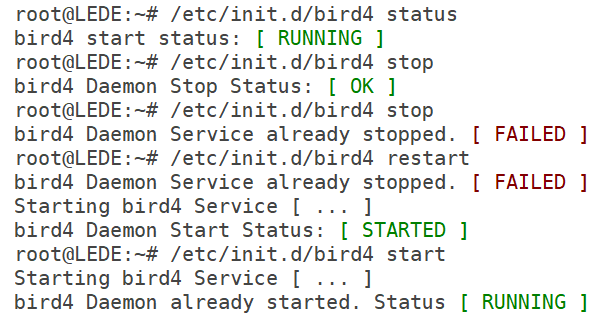
\includegraphics[width=0.7\textwidth]{images/initdterminal}
    \caption{Service management for Terminal.}
    \label{fig:initdt}
\end{figure}

\begin{figure}[ht!]
    \centering
    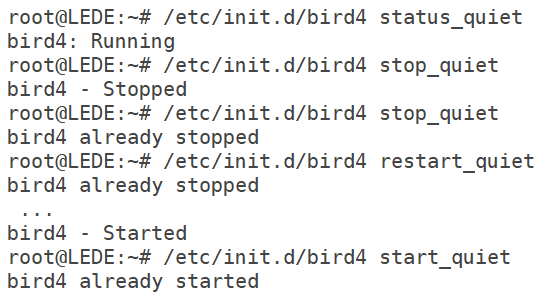
\includegraphics[width=0.7\textwidth]{images/initdui}
    \caption{Service management for Web UI.}
    \label{fig:initdui}
\end{figure}

\subsection{UCI Configuration improvements}
\label{sec:uciimp}
The Unified Configuration Interface (UCI) aims to centralise OpenWrt's settings and it is widely used for almost, if not all, the packages in OpenWrt. UCI allows you to easily, and in a human-readable manner, configure any system following the same scheme, simplifying administration overheads.

However, \textit{bird-uci} Package uses the UCI configuration file in a non-classical manner. Instead of making use of the configuration as it is, the Package only acts as a translator between what the user wants (written in UCI-scheme) and what bird needs to work (c-like configuration file). As stated in section \ref{sec:motivation}, the first version of the package successfully manages Bird, but there have been some API changes since Bird v1.4.3 and the integration is not completed yet:

\begin{itemize}
    \item As part of Bird's v1.4.3 to v1.6.3 API reviewing, some options have required tweaking in order to be compliant to the latest API.
    \item Most of the UCI improvements are tied to LUCI improvements (see section \ref{sec:luciimp}) in order to enhance User eXperience.
    For example, BGP Protocol allows you to execute an action once a number of routes is reached (imported, exported or received). This is shown as a pair of settings in the UI. Previously, each setting was independent, which was a problem as both are optional and hidden for simplicity reasons.
    By adding the extra option, I have been able to tie both options graphically and make them work as expected.
    From /etc/config/bird4:
    \begin{lstlisting}[language=bash,caption={Tied options using UCI (I)}]
config bgp 'bgpAS1'
        option import_trigger '0'
        option export_trigger '0'
        option receive_trigger '0'
        option disabled '0'
        option template 'test123'
        option neighbor_address '192.168.1.100'
        option neighbor_as '1'
\end{lstlisting}

    As shown in the snippet, we have three \texttt{\_trigger '0'} options that states that there is \textbf{no} Limit set in this BGP session. However, if we set one through the UI:
    \begin{figure}[H]
    \centering
    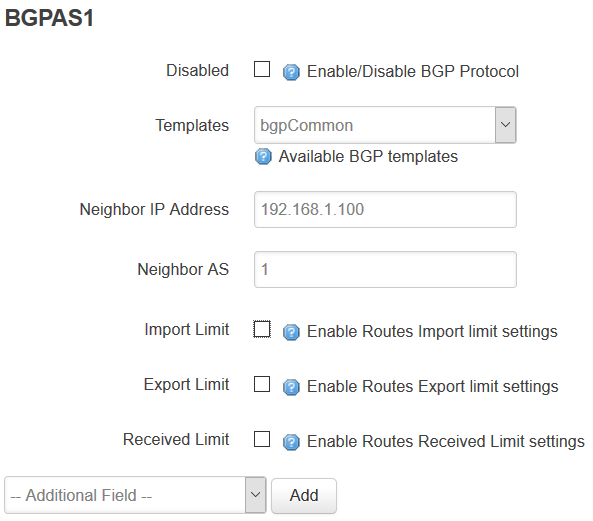
\includegraphics[width=0.8\textwidth]{images/bgp/bgptrigger1}
    \caption{Import Limit Trigger \textbf{not} selected.}
    \label{fig:uitiedn}
\end{figure}

\begin{figure}[H]
    \centering
    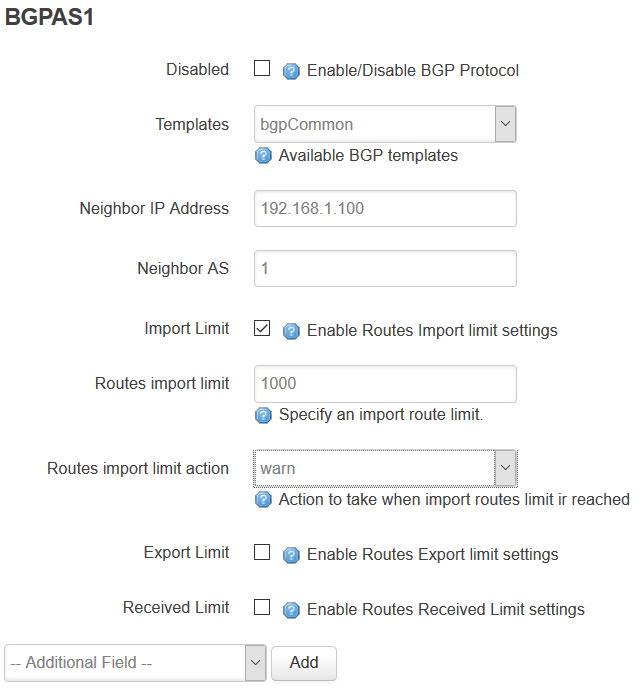
\includegraphics[width=0.8\textwidth]{images/bgp/bgptrigger2}
    \caption{Import Limit Trigger \textbf{selected}.}
    \label{fig:uitiedy}
\end{figure}

As shown in both figures \ref{fig:uitiedn} and \ref{fig:uitiedy} LUCI brings both options together, making it clear to the administrator that these settings must be filled. The UCI result for \ref{fig:uitiedy} is the following:

\begin{lstlisting}[language=bash,caption={Tied options using UCI (II)}]
config bgp 'bgpAS1'
        option import_limit_action 'warn'
        option export_trigger '0'
        option receive_trigger '0'
        option disabled '0'
        option template 'bgpCommon'
        option neighbor_address '192.168.1.100'
        option neighbor_as '1'
        option import_trigger '1'
        option import_limit '1000'
\end{lstlisting}

This \textit{tying} improvement has been done in the web UI's and not in UCI translation time because, as can be seen in the following code snippet, it is easier to let LUCI configuration management process to add/remove those attributes automatically on settings save time, than doing some hand-made if statements.

In the following LUA snippet, LUCI creates a UI Flag option (our trigger) which is mandatory (\texttt{optional = false}. The other two options (\texttt{limit} and \texttt{limit\_action}) are both optional and dependant on the value of our flag (\texttt{depends({import\_trigger = "1"})}.

\begin{lstlisting}[language=lua, caption={LUCI tied options implementation.}]
[...]
import_trigger = sect_templates:option(Flag, "import_trigger", "Import       Limit", "Enable Routes Import limit settings")
import_trigger.default = 0
import_trigger.rmempty = false
import_trigger.optional = false

import_limit = sect_templates:option(Value, "import_limit", "Routes import   limit", "Specify an import route limit.")
import_limit:depends({import_trigger = "1"})
import_limit.rmempty = true

import_limit_action = sect_templates:option(ListValue,                       "import_limit_action", "Routes import limit action", "Action to take when    import routes limit ir reached")
import_limit_action:depends({import_trigger = "1"})
import_limit_action:value("warn")
import_limit_action:value("block")
import_limit_action:value("disable")
import_limit_action:value("restart")
import_limit_action.default = "warn"
import_limit_action.rmempty = true
[...]
\end{lstlisting}
\end{itemize}

\newpage

\subsection{LUCI UI improvements}
\label{sec:luciimp}
Following previous section \ref{sec:uciimp} UCI/LUCI example, there have been other UI improvements coupled with changes in the UCI implementation. The following subsections will cover each UI Page to summarise its role and which changes have been done to it. Nevertheless, the last subsection will explain the number of challenges faced during project's development.

\subsubsection{Status Page}
\textbf{New} Page allowing an administrator to manage Bird Service. This page shows 3 buttons tied with the init.d functions explained in section \ref{sec:initd} figure \ref{fig:initdui}.


The contents of this page are:
\begin{itemize}
    \item Three buttons to trigger the service management: Start, Stop and Restart in Quiet mode.
    \item Dynamic Text Box showing Bird service's status. This text will be updated if you trigger any service update through the buttons.
\end{itemize}

\begin{figure}[H]
    \centering
    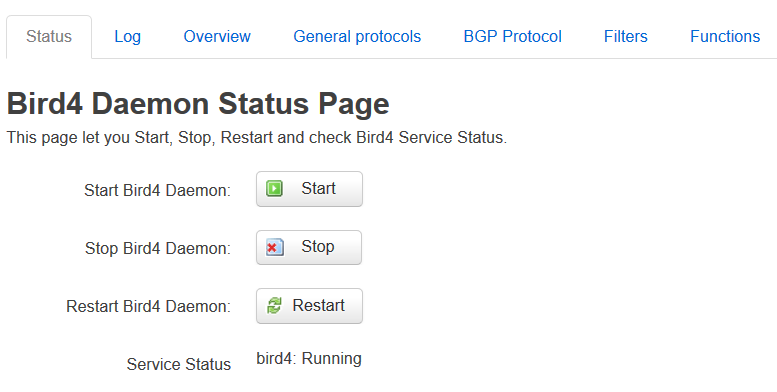
\includegraphics[width=0.8\textwidth]{images/bird0.3/status}
    \caption{Status Page}
    \label{fig:statusp}
\end{figure}

Although contents of this page are simple and straightforward, the result shown in figure \ref{fig:statusp} is not the desired one. The initial idea was to use a single button for starting and stopping the service, and none for restart. Moreover, the button would be automatically switch between states showing, when started, service's PID. In Appendix \ref{app:ch:extrap} you can see the expected behaviour shown in the LUCI implementation of Privoxy's OpenWrt Package.

The reason behind not doing it is that this simple change would require to change from using LUCI's CBI (Lua) to LUCI2 (JavaScript). Lua's implementation allows you to trigger a number of actions according to a specific element state, if an action (i.e. button clicked) is triggered or during page's rendering. However, there is no granular control on it or a polling mechanism that could automate the transition between service disabled and enabled. To do so, it would be required to force the page to wait (manual OS \texttt{sleep} command) which would also \textbf{block} page's loading.

Moreover, I did do a test implementation (without a \texttt{sleep}) and, because of the way CBIs work, the button action and rendering action were somehow triggering service calls multiple times, starting and stopping the service in an unexpected way and not refreshing the contents (wrong status and PID displayed).

\subsubsection{Log Page}
\textbf{New} Page showing contents in Bird's configured Log file. This page is automatically refreshed \textbf{each second} with the following information:

\begin{itemize}
    \item Name of the Log file. For reference and easier administration.
    \item Size of the Log file. Critical information in Bird configurations where \textbf{Debug} information is also enabled. Log file can grow really fast if there are more peers sharing information or if the debug mode is set to log most/all the possible events in the system.
    If the Log file grows enough to fill the /var partition, Bird will \textbf{automatically} shutdown and \textbf{prevent} any start up attempt until this is resolved. 
\end{itemize}

\begin{figure}[H]
    \centering
    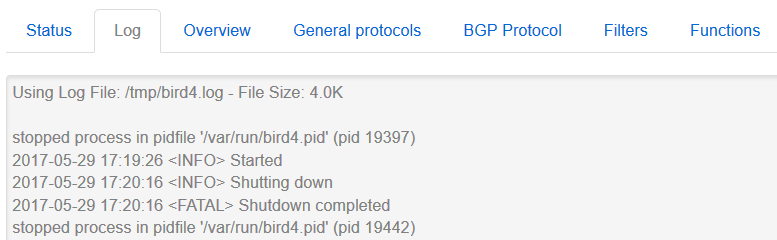
\includegraphics[width=\textwidth]{images/bird0.3/log}
    \caption{Log Page: service restart example}
    \label{fig:statusp}
\end{figure}

This page has been implemented using mixed capabilities from LUCI and LUCI2. Because of the requirement to show a \textbf{rolling} Log page with a reasonably regular auto-refresh process, it was necessary to use JavaScript's XHR capabilities embedded in the HTML page itself together with Lua code to read the file and send the text as a PlainText HTML response (object).

Because of the lack of documentation in this area, I did spend weeks investigating it by my own using the available package sources in OpenWrt's repositories. However, because what the other packages usually do is to use XHR polls as a communication broker method (i.e. get a specific data from a specific UCI file, apply some filtering/transformation if the data is not in the desired state and, finally, populate specific UI fields available in the HTML page) it was not clear what exactly I had to do as I only needed to: read last 30 lines of a file (Bird's Log File) and populate the Text View (Plain text data).

Finally, after spending some days trying to contact experienced LEDE/OpenWrt developers using community's contact channels\footnote{LEDE community contact methods: \href{https://lede-project.org/contact}{Link}}, I could have few conversations with one of the main contributors of LEDE, OpenWrt \texttt{jow-}\footnote{Jo-Philip Wich: \href{https://github.com/jow-}{Github Profile}.} and also main author of LUCI/LUCI2, who gave me some hints and examples of LUCI2 pages that helped me fixing my issues with the Log and Filters/Functions pages.\\

\textbf{Log File key elements:}
\\
Only execute the polling function if \textit{refresh} is passed as parameter.
\begin{lstlisting}[language=lua]
if luci.http.formvalue("refresh") then
\end{lstlisting}

Send the outputs back as plain text.
\begin{lstlisting}[language=lua]
luci.http.prepare_content("text/plain")
\end{lstlisting}

Get the last 30 lines of the file \texttt{log\_file}
\begin{lstlisting}[language=lua]
lf = sys.exec("tail -n30 " .. log_file):gsub("\r\n?", "\n")
\end{lstlisting}

Send, as HTTPResponse object, the quoted message.
\begin{lstlisting}[language=lua]
luci.http.write("Using Log File: " .. log_file .. " - File Size: " .. log_size .. "\n" .. lf)
\end{lstlisting}



\subsubsection{Service Overview Page}

\subsubsection{General Protocols Page}

\subsubsection{BGP Protocol Page}

\subsubsection{Filters \& Functions Page}

\subsection{Align documentation and upgrade to Markdown}

\newpage
\section{Package Testing}
Testing an integration/translation Package, and this one specifically, is a rather complex task to evaluate as Bird configuration files are modular and desired settings can be achieved in different ways. Even more, although a \textit{it works/it does not work} policy could be accepted, it does not mean that there are not other possible implementations that could work in a better way. For example, filters and functions can be either written in the \textit{.conf} file or included using \textbf{\%include} mechanism, being the second one a better approach as it enhances code readability as well as it avoids bloating the configuration file unnecessarily.

With this introduction in mind, the following sections will explain how this package has been tested following Bird's configuration base requirements and service behaviour and some \textit{future work} ideas to achieve automatic and unit tests.


\subsection{Configuration Translation Tests (future work)}
To perform configuration integrity tests in current package, it is required to repeat the execution of \texttt{/etc/bird\{4|6\}/init.d/bird4 restart} in order to trigger the UCI-bird.conf translation from a target UCI file. The code to do this translation has been refactored in an functional manner to allow future unit tests or, at least, make it easier to integrate in an automated test framework or process. For example, an automated CI/CD build process could build an update of the package, push it into a test node, execute the translation process and compare it against the previous (or a stable) version as well as check its correctness by querying Bird's status.

\subsubsection{Reviewing v0.2 against v0.3}
Testing the outputs from the old and new packages, and taking into account that there are some manual changes in the old one, the following example is configured as follows:

\begin{itemize}
    \item Router IDs follow node's IP Address
    \item Kernel, Device and Static Protocols have been set by default
    \item A Static Route has been added  (identical)
    \item BGP Template and Instance have been configured following v0.2 scheme with matching settings to avoid Bird failures
    \item BGP Instance AS and Neighbours are dummy values
    \item A BGP Filter called "all\_ok" (accept all routes) has been added using each version's process.
\end{itemize}

In the new package, we have instantaneous configuration correctness feedback as we can check Bird's status in the Status Page. 
In the old package, after executing \texttt{/etc/bird\{4|6\}/init.d/bird4 start}, Bird will fail and it is required to move the Filter "all\_ok" to the top of the document. Bird will start correctly after this modification.

After checking that both daemons are running, we can then perform a \textit{diff} between the configuration files and look for any noticeable difference

\begin{lstlisting}[language=diff,caption={Differences in Bird configuration using v0.2 and v0.3 of the Package.}]
3,9d2
<    #Filter filter1:
<    filter all_ok
<    {
<        accept "all ok";
<    }
<
13c6
<    router id 192.168.1.200;
---
>    router id 192.168.1.100;
17a11,17
>    #Functions Section:
>    #End of Functions --
>  
>    #Filters Section:
>    include "/etc/bird4/filters/filter1";
>    #End of Filters --
>  
19c19
<    protocol kernel {
---
>    protocol kernel kernel1 {
46c45
<    source address 192.168.1.200;
---
>    source address 192.168.1.100;
57c57
<    neighbor 192.168.1.201 as 1002;
---
>    neighbor 192.168.1.101 as 1002;
\end{lstlisting}

As shown in this \textit{diff} snippet, almost all the translated configuration is identical apart from:

\begin{itemize}
\item Different Router IDs and BGP neighbours (expected)
\item Kernel Protocol definition (minor change in the API)
\item BGP Filter definition (major change in the API)
\end{itemize}

\subsection{Bird Daemon Errors}
Bird Daemon provides an error exit code together with different text outputs in order to highlight errors in the configuration. Although most of the times it can be easily spotted using Bird's feedback, there are also instances where the Daemon's documentation may be required to fix them.

\subsubsection{Bird Daemon Error examples}
Most common errors that an administrator may need to resolve are:

\begin{itemize}
\item A configured field has incorrect syntax.
Bird will give you hints about what is wrong most of the times: wrong IP address format \texttt{bird: /tmp/bird4.conf, line 7: Invalid IPv4 address 1921.68.1.1}. But some \textit{rare} times the message is less helpful and you may need to check the contents of the file and understand the error.

As an example of this: \texttt{bird4: Failed - bird: /tmp/bird4.conf, line 65: syntax error}. We need to check the bird4.conf file and see that in line 65:

\begin{lstlisting}[language=bash, caption={Bird4.conf contents}]
64:    protocol bgp BGPExample {
65:        import Filter NonExistingFilter;
66:    }
\end{lstlisting}

We will need to find out that the shown filter used in the \textbf{import} field of BGP Protocol, does not exist.

\item Non-compatible configuration.
The other set of common errors is non-compatible fields in a Protocol.

As an example of this: \texttt{bird: /tmp/bird4.conf, line 76: Only internal neighbor can be RR client}. We need to remove the Route Reflector Client setting from the BGP Instance to fix this behaviour.

\item Missing filter or function
If you include a filter name in any of the Protocols or if any of your filters use a non-existing function, Bird will fail to start showing an error as follows: \texttt{bird: /tmp/bird4.conf, line 71: No such filter}.

\item Syntax errors in a filter or function.
This error follows the same approach as the first bullet: \texttt{bird: /etc/bird4/filters/filter-20170507-0951, line 4: syntax error}. You are required to go to command line and fix the problem checking the configuration and filter or function files.

\item Filter calling to non-existing functions.
If your filter executes a command that is not defined by Bird's syntax, it will handle it as a function. If that function does not exist in any of the handled files, it will show this error: \texttt{bird: /tmp/bird4.conf, You can't call something which is not a function. Really.}

\item Filters not accepting/rejecting routes.
Bird Daemon filters must return an \textit{accept} or \textit{reject} policy per route received. If any of your filters does not return any policy per route, it will be silently ignored and substituted with an "accept".

As an example of this issue:
\begin{lstlisting}[language=bash, caption={Filter printing message}]
filter doNothing
{
    print "HelloWorld";
}
\end{lstlisting}

Bird Daemon will succeed starting up but, if we check the log information in the Log Page, this error message will be shown:
\begin{lstlisting}[language=bash, caption={Filter printing message.}]
<ERR> Filter doNothing did not return accept nor reject. Make up your mind
<INFO> HelloWorld
\end{lstlisting}

\end{itemize}

\subsection{Real Scenario: VM with simple BGP configuration connected to Guifi.net}
As part of the acceptance tests, a VM was set up by a sysadmin in the \textit{Universitat Oberta de Catalunya} to act as a pre-production machine. This VM is connected to a \textit{Mikrotik} Router acting as Gateway to \textit{Guifi.net} but this scenario does \textbf{not} connect or communicate through any Mesh Network using BMX6, so it is an end point.

The configuration of this system is almost identical, component-wise, to the ones available in Guifi.net. However, this system will only route itself (1 route) and import any.

Bird UCI configuration set through the WEB UI and its translation into Bird4 configuration can be reviewed in appendix \ref{app:ch:bdcuoc}.

This VM is communicating to Guifi.net through a Mikrotik which is already doing some filtering but, in any case, it is still able to import 3000+ Routes and export itself:

\begin{lstlisting}[language=bash,caption={Bird BGP query.}]
root@LEDE-eloi:~# birdcl4 show protocols all
[...]
BGPImportALL BGP      master   up     2017-05-10  Established
  Preference:     100
  Input filter:   ebgp_in
  Output filter:  ebgp_out
  Import limit:   3000 [HIT]
    Action:       warn
  Routes:         2999 imported, 1 exported, 2999 preferred
  Route change stats:     received   rejected   filtered    ignored   accepted
    Import updates:        1208383          0          0         88    1208295
    Import withdraws:       337268          0        ---        300     336968
    Export updates:        1208298    1208295          2        ---          1
    Export withdraws:       336968        ---        ---        ---          0
  BGP state:          Established
    Neighbor address: 172.25.35.25
    Neighbor AS:      59361
    Neighbor ID:      10.90.224.65
    Neighbor caps:    refresh AS4
    Session:          external AS4
    Source address:   172.25.35.26
    Route limit:      2999/3000
    Hold timer:       160/180
    Keepalive timer:  29/60
\end{lstlisting}

Using Bird Lightweight Remote Control (\textbf{birdcl4}) we can verify Bird's BGP instance. As key information:

\begin{itemize}
    \item BGP Instance: BGPImportALL
    \item Filters applied: \textit{ebgp\_in} and \textit{bgp\_out}
    \item We are connected to our neighbour 10.90.224.65 with Autonomous System ID 59361
    \item  The number of routes received fluctuates but the data shown presents 2999 routes imported.
    \item We do not know when, but the import Limit reached (HIT) and that generated warnings.
    From our Package's Log Page:
    \texttt{2017-05-21 22:09:13 <WARN> Protocol BGPImportALL hits route import limit (3000), action: warn}
    \item We are exporting 1 Route.
\end{itemize}

As a health check, we can query Bird of its last reconfiguration, reboot time or status using \texttt{bircl4 status}:

\begin{lstlisting}[language=bash,caption={Bird status query.}]
root@LEDE-eloi:~# birdcl4 show status
BIRD 1.6.3 ready.
BIRD 1.6.3
Router ID is 10.139.173.161
Current server time is 2017-05-22 00:20:23
Last reboot on 2017-05-10 19:31:09
Last reconfiguration on 2017-05-10 19:31:09
Daemon is up and running
\end{lstlisting}
